\subsection{Social-LSTM: deterministic social pooling}
\label{sec:social_lstm}
\paragraph{Implementation and paper correspondence.}
WANG Yifan independently implemented a deterministic adaptation of Social-LSTM for the group's registered $K=1$ comparison. The original architecture exchanges recurrent information through a spatial social-pooling grid \cite{alahi2016social}. Our model embeds two-dimensional displacement, pools neighboring hidden states in a $4\times4$ grid covering a 4\,m square, and updates a shared LSTM with hidden size 64 and embedding size 32. Self-connections and padding are excluded. A neighbor is eligible only if all eight observed positions exist and its distance from the target is at most 6\,m at some observed time. Future track availability never determines this eligibility.

The model jointly rolls all admitted actors forward for twelve steps from eight observations at 0.4\,s spacing. Its deterministic displacement equals the fixed mean of the last three observed displacement intervals plus a learned recurrent residual. The history-derived anchor stays fixed throughout rollout. A target-relative origin is removed internally and added back to predictions. Neighbor positions receive no benchmark corruption; target-relative geometry is recomputed after target corruption.

This is a group-specified deterministic variant, not an exact numerical reproduction of the paper's Gaussian position model. The output head, displacement anchor, hidden/grid dimensions and training objective are declared adaptations. Unlike the earlier exploratory $K=20$ implementation, it has no Gaussian sampling or teacher forcing and does not feed sampled innovations into a persistent velocity baseline. The preserved exploratory results are excluded from the shared table. Because architecture, loss, training splits and seed settings changed together, their difference cannot isolate the effect of any single modification.

\paragraph{Training, selection and verification.}
All five folds use the unchanged shared ordered manifests and seeds 0/1/2. We trained each of the 15 runs for a predeclared 12 epochs using Adam (learning rate $10^{-3}$, weight decay $10^{-4}$), gradient clipping at 10 and batches of 32. Actor-count bucketing reduces padding while visiting every training window once per epoch. The loss is mean squared target-position error over the full closed-loop forecast. Clean-validation ADE selects one checkpoint, with the earlier epoch breaking ties; the same checkpoint serves all six test conditions.

The common setup gate and separate full-population ETH seed-0 pilot passed before formal training. Owner tests check target/neighbor future-coordinate and stored-derivative invariance, future-presence invariance, exact target-only perturbation seeds, causal missing-suffix filling, coordinate round-trip, padding isolation, social-grid gradients and deterministic $K=1$ output. The common auditor verifies all 90 bundles, their ordered IDs, observations, masks, labels and configuration/checkpoint hashes, and independently recomputes the headline scores. This interface audit does not replace editor review of the implementation and artifact reproduction.

\paragraph{Shared results.}
\begin{table}[ht]
\centering\small
\caption{Social-LSTM shared $K=1$ fold macros in meters. At $K=1$, minimum and mean ADE/FDE coincide and sample diversity is zero.}
\label{tab:social_lstm-causal}
\begin{tabular}{lrr}\toprule
Condition & ADE & FDE \\\midrule
Clean & \ModelMetric{social_lstm}{clean_0}{mean_ade_mean} & \ModelMetric{social_lstm}{clean_0}{mean_fde_mean} \\
Noise 0.05\,m & \ModelMetric{social_lstm}{noise_005}{mean_ade_mean} & \ModelMetric{social_lstm}{noise_005}{mean_fde_mean} \\
Noise 0.10\,m & \ModelMetric{social_lstm}{noise_010}{mean_ade_mean} & \ModelMetric{social_lstm}{noise_010}{mean_fde_mean} \\
Noise 0.20\,m & \ModelMetric{social_lstm}{noise_020}{mean_ade_mean} & \ModelMetric{social_lstm}{noise_020}{mean_fde_mean} \\
Missing 1 & \ModelMetric{social_lstm}{missing_1}{mean_ade_mean} & \ModelMetric{social_lstm}{missing_1}{mean_fde_mean} \\
Missing 2 & \ModelMetric{social_lstm}{missing_2}{mean_ade_mean} & \ModelMetric{social_lstm}{missing_2}{mean_fde_mean} \\\bottomrule
\end{tabular}
\end{table}

Clean macro ADE is $0.607\pm0.014$\,m and FDE is $1.232\pm0.024$\,m. The uncertainty shown is sample standard deviation across three seed-wise equal-scene macros, not a confidence interval. Constant velocity, using the last observed displacement on the identical test manifests, achieves 0.534\,m ADE. Our learned variant's error is 13.7\% higher; this is a descriptive fixed-budget comparison, not a controlled attribution to social pooling. Clean RMS-norm Energy Score is 0.721\,m. At 0.20\,m target noise ADE is 1.128\,m, and with two missing positions it is 0.761\,m. The selected epochs have median 1, consistent with validation curves favoring early checkpoints over continued reduction of training loss.

\begin{figure}[ht]
\centering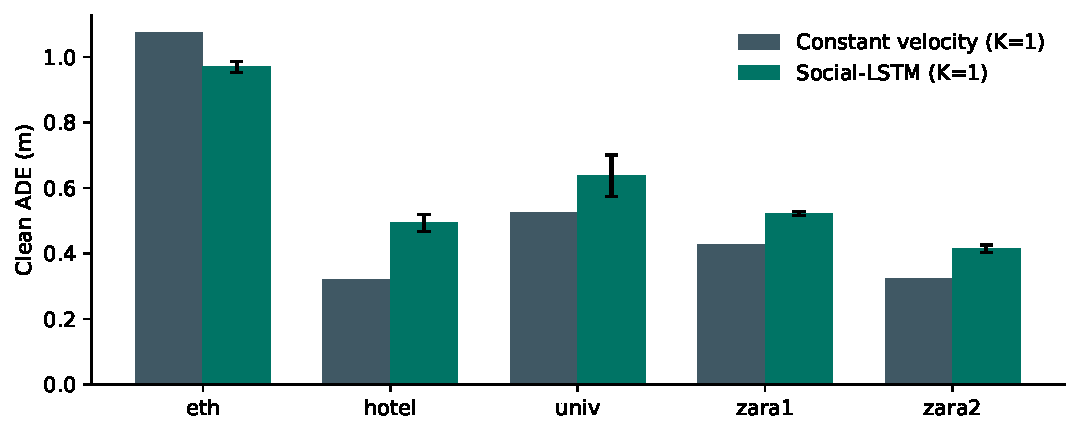
\includegraphics[width=.80\linewidth]{contributions/social_lstm/evidence/causal_clean_accuracy.pdf}
\caption{Clean fold errors against last-displacement constant velocity on the identical shared test manifests. Bars on Social-LSTM indicate sample standard deviation across three seeds, not confidence intervals.}
\label{fig:social_lstm-clean}
\end{figure}

\paragraph{Crowded and turning trajectories.}
For descriptive analysis, a crowded window has at least five admitted observed neighbors. Its clean ADE macro is 0.631\,m, compared with 0.596\,m for fewer neighbors. Turning windows have at least a 30-degree change between the observed and final-future three-interval mean directions, with both speeds at least 0.3\,m/s. Their ADE is 1.105\,m versus 0.553\,m for the remaining windows. These unpaired subsets differ in motion and scene composition, so the gaps do not isolate the causal effect of density or turning. Group counts and fold/seed values are retained with the evidence.
The qualitative example is selected by the largest truth-defined direction change among the fixed Hotel runtime IDs with both observed and late-future speed at least 0.3\,m/s. Selection uses neither prediction error nor checkpoint performance. It illustrates one turning case and is not a representative sample.
\begin{figure}[ht]
\centering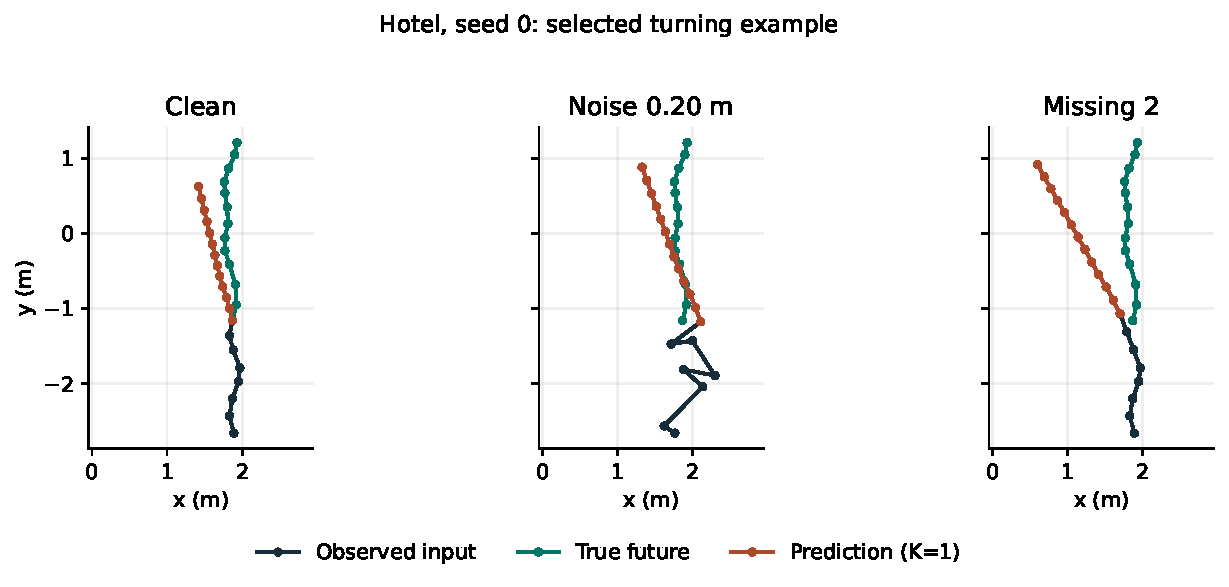
\includegraphics[width=.95\linewidth]{contributions/social_lstm/evidence/causal_turning.pdf}
\caption{The same Hotel seed-0 checkpoint under clean, 0.20\,m target noise and two missing observations. Observed input, true future and one deterministic forecast are shown in metric coordinates.}
\label{fig:social_lstm-turning}
\end{figure}

\paragraph{Runtime, reproducibility and limits.}
The 15 runs required 86.3 minutes of recorded training/validation time. Standard runtime measurements use 128 ordered targets, four batches of 32, three warmups and ten repetitions for each fold/seed. Averaging the per-run medians gives 2.5\,ms preprocessing, 44.9\,ms deterministic prediction and 48.4\,ms end-to-end. The boundary starts from cached neutral metric histories, includes neighbor filtering, padding, device transfer and metric CPU output, and excludes disk loading, initial window caching and scoring. Process-lifetime peak RSS reached 1023\,MiB; this is not a GPU peak-memory measurement.
Training and prediction used Apple M5 MPS with Python 3.13.12, PyTorch 2.11.0 and NumPy 2.4.4. This differs from the repository's Linux x86-64 reference environment. Hardware-specific timing must be presented separately, and reference-environment reproduction and final readiness remain editor review items. The release retains weights, full prediction bundles, validation-selection tables and timing repetitions locally with a recorded archive SHA-256. Git contains portable sources and lightweight evidence. Code, source inventory and disclosed AI assistance accompany the model.
